\tunemarkup{pghanlin}{\newcommand{\coverimagescale}{1.67}}
\tunemarkup{pgkoboaurahd}{\newcommand{\coverimagescale}{1.89}}
\tunemarkup{pgnexus7}{\newcommand{\coverimagescale}{1.71}}
\tunemarkup{pgkindledx}{\newcommand{\coverimagescale}{2.7}}
\tunemarkup{pgkobomini}{\newcommand{\coverimagescale}{1.67}}

\tunemarkup{coverimage}{%
\newpagecolor{ubpagecolor}\afterpage{\restorepagecolor}
\begin{center}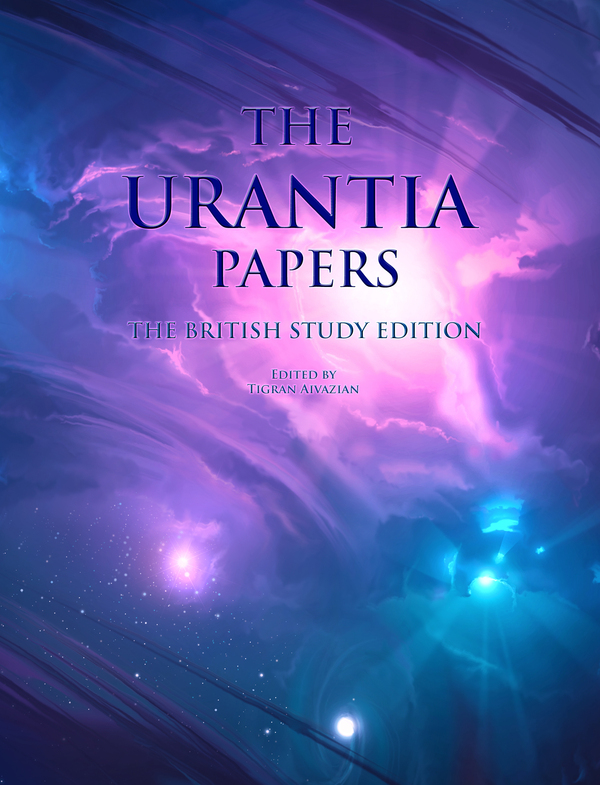
\includegraphics[scale=\coverimagescale]{images/British-Study-Edition-Cover-tiny.jpg}\end{center}
\newpage
}

\makeatletter
\bib@raise@anchor{\bibpdfbookmark[0]{Title Page}{Ttl}}%
\makeatother

\vspace*{\stretch{0.01}}
\begin{center}
{
\bibcovertitlefont
\tunemarkup{pgkindledx}{\fontsize{20.8}{32}\selectfont}
\tunemarkup{pghanlin}{\fontsize{12}{20}\selectfont}
\tunemarkup{pgkobomini}{\fontsize{14}{20}\selectfont}
\tunemarkup{pgnexus7}{\fontsize{13.5}{20}\selectfont}
\tunemarkup{pgkoboaurahd}{\fontsize{15}{20}\selectfont}
THE BRITISH \tunemarkuptwo{nofnt}{TEXT}{STUDY} EDITION\\
\tunemarkup{pgkindledx}{\fontsize{16.5}{32}\selectfont}
\tunemarkup{pghanlin}{\fontsize{9}{20}\selectfont}
\tunemarkup{pgkobomini}{\fontsize{10}{20}\selectfont}
\tunemarkup{pgnexus7}{\fontsize{10}{20}\selectfont}
\tunemarkup{pgkoboaurahd}{\fontsize{12}{20}\selectfont}
{\itshape OF}\\
\tunemarkup{pgkindledx}{\fontsize{16.2}{32}\selectfont}
\tunemarkup{pghanlin}{\fontsize{9}{20}\selectfont}
\tunemarkup{pgkoboaurahd}{\fontsize{11.8}{20}\selectfont}
\tunemarkup{pgkobomini}{\fontsize{11}{20}\selectfont}
\tunemarkup{pgnexus7}{\fontsize{10.6}{20}\selectfont}
{\itshape THE FIFTH EPOCHAL REVELATION}\\
}%
{%
\vspace*{\stretch{0.1}}
\tunemarkup{pghanlin}{\fontsize{10}{13}\selectfont}
\tunemarkup{pgkindledx}{\fontsize{16}{18}\selectfont}
\tunemarkup{pgnexus7}{\fontsize{10}{12}\selectfont}
\tunemarkup{pgkoboaurahd}{\fontsize{13}{15}\selectfont}
\itshape
The Standard Reference Text in British English\tunemarkuptwo{nofnt}{\\[2ex]}{%
,\\
with Metric Measures, Textual Variants,\\
Study Notes \&\ \totalfigures\ Illustrations\\[2ex]
}
\tunemarkup{pgnexus7}{\textcolor{ubdarkred}{With Words of Jesus in Red Colour}\\[1pt]}
Edited by Tigran Aivazian\\[2ex]
\tunemarkuptwo{noquiz}{}{With Interactive Cosmic Citizenship Quiz\\(\totalcurqs\ questions in total)\\}
}%
\vspace*{\stretch{0.6}}
\tunemarkuptwo{nofancydecor}{}{%
\titlesepbig\\
}
\vspace*{\stretch{0.1}}
\end{center}

\tunemarkuptwo{nofancydecor}{}{\titleframe}

\newpage

%\newcommand{\serpimolot}{{\fontspec{Mortbats} K}}

\begin{center}
\vspace*{\stretch{0.3}}
\begin{center}\shadowbox{\strut\parbox{7cm}{\tunemarkuptwo{pgkindledx}{\Large}{\large}\bfseries\itshape ``Of all human knowledge, that which is of greatest value is to know the religious life of \mbox{Jesus} and how he lived it.'' \bibref[(196:1.3)]{p196 1:3}}}\end{center}
\vspace*{\stretch{0.5}}
\tunemarkup{pghanlin}{\fontsize{8}{10}\itshape}
\tunemarkup{pgnexus7}{\fontsize{8}{10}\itshape}
\tunemarkup{pgkindledx}{\fontsize{10}{12}\itshape}
\parbox{0.9\linewidth}{\centering
\textbf{\upshape\nocopyright\ No copyright is claimed on this book\\
The text of the Urantia Papers is in the public domain}.\\[5pt]
\tunemarkuptwo{coverimage}{Cover design by Gary Tonge, www.vision-afar.com.\\}{}
The latest version of this book can be downloaded from:\\
{\upshape\bfseries http://www.bibles.org.uk}\\
Please send all comments \&\ suggestions to {\makeatletter\upshape\bfseries aivazian.tigran@gmail.com\makeatother}\\
\tunemarkuptwo{nofnt}{}{The apparatus (marked with a circle in the text) contains all significant changes made since the 1955 first edition.\\}
The symbol \pc\ marks the first paragraph in the group as in the first edition, where such groups were delimited by blank lines.\tunemarkuptwo{nofnt}{\\[5pt]}{ The asterisk * indicates a study note other than a textual variant.\\[5pt]}
\tux\ Typeset with \XeLaTeX\ under Linux.\\
Text set in \textbf{\itshape\tunemarkup{minionpro}{Adobe }\tunemarkup{garamond}{Adobe }\tunemarkup{arno}{Adobe }\tunemarkup{academy}{ParaType }\urantiamainfont} at \urantiamainfontsize pt.\\[18pt]
\upshape\small\bfseries PDF version: \tunemarkup{pgnexus7}{7in Colour}\tunemarkup{pghanlin}{6in eInk}\tunemarkup{pgkobomini}{5in eInk}\tunemarkup{pgkoboaurahd}{7in eInk}\tunemarkup{pgkindledx}{10in eInk}\\
\upshape\small\bfseries PDF date: \mytoday{}\\
}
\end{center}

\tunemarkuptwo{nofancydecor}{}{\titleframe}
